% !TEX root = ../thesis_main.tex



%%%% --- * --- %%%%	
\clearpage
%\part{Background}
%\chapter{Motivation}

\chapter{Background and Motivation}
\label{background_chapter}

\section{Exotic Couplings}
	In particular, we're interested in so-called scalar and tensor couplings within the nuclear weak force. Standard model beta decay involves only vector and axial-vector couplings.
		
\section{Fierz Interference -- The Physical Signature}
	The physical effects resulting from the presence of scalar or tensor couplings include a small perturbation to the energy spectrum of betas produced by radioactive decay.  
		
\section{Present Limits}
	A bit about other people's physics.
	
\section{A Toy Experiment}
	A quick overview of how an experiment like this one would be set up to extract the physics of interest, to keep the reader from getting too lost in the rest of the thesis.


%%%% --- * --- %%%%	
\clearpage
\chapter{Theoretical Overview}
\label{theory_chapter}

\section{The Basics of Beta Decay}
	%\\*
	Standard model beta decay is well understood.  The Fermi model of beta decay is in all the textbooks, but you have to dig slightly harder to understand Gamow-Teller or mixed decays, all of which are relevant here.
	
\section{JTW Formalism}	
	%\\*
	Describes how to search for a variety of BSM terms within beta decay.  Does not account for certain well-understood effects of similar (or greater) magnitude.
	
\section{Holstein Formalism}
	%\\*
	An in-depth mathematical description of beta decay, including many smaller effects.  It does not include a description of the BSM physics of greatest interest to us.   
	
\section{Relation between JTW and Holstein Formalisms}
	%\\*
	To conduct a precision search for scalar and tensor couplings, it is necessary to combine the Holstein and JTW models into a single cohesive probability distribution.  


%%%% --- * --- %%%%	
\clearpage
%\part{Experimental Overview}
\chapter{The Experimental Setup}
\label{setup_chapter}

\section{Double MOT System to Supply Atoms}
	%\\*
	Mostly, 
	\margintodo{A thing that's worth noting is that (I think!) recoil-order corrections have been implicitly excluded at some point here.  ...Is this even true??}
	this requires a diagram.  We take ions supplied by the ISAC beamline, neutralize them and trap them in the first MOT, then periodically transfer them to a second MOT.  Detectors are 
%	\todo{A thing that's worth noting is that (I think!) recoil-order corrections have been implicitly excluded at some point here.  ...Is this even true??}
	positioned about the second MOT for data 
%	\lefttodo{A thing that's worth noting is that (I think!) recoil-order corrections have been implicitly excluded at some point here.  ...Is this even true??}
	collection.  This double MOT system eliminates a great deal of background.  
%	\tinytodo{A thing that's worth noting is that recoil-order corrections have been implicitly excluded at some point here. (Here's a parenthetical.) ...Is this even true??  Also, what is even happening to the spacing here??!}
	Also, here's some random equation that doesn't really go with the topic of this section:
	\bea
\frac{\partial \rho}{\partial t} &\!\!\!\!\!\! \bigg|_{relax} \!\!\! &= \:\:\: -\frac{1}{2} \left( \hat{\Gamma} \rho + \rho \,\hat{\Gamma} \right) 
\label{eq:relax} \\
\frac{\partial \rho}{\partial t} &\!\!\!\!\!\!  \bigg|_{repop} \!\!\! &= \:\:\: \hat{\Lambda},
\label{eq:repop} 
\eea

	Furthermore, here's a picture that doesn't really go with the topic of this section.
%	\lefttodo{A thing that's worth noting is that (I think!) recoil-order corrections have been implicitly excluded at some point here.  ...Is this even true??}
	collection.  This double MOT system 
%	\margintodo{A thing that's worth noting is that (I think!) recoil-order corrections have been implicitly excluded at some point here.  ...Is this even true??}
	eliminates a great deal of background.  
	
	
\section{AC-MOT and Polarization Setup}
	%\\*
	In order to facilitate a measurement of $A_{\mathrm{\beta}}$, we went to great efforts to polarize the atom cloud, and quantify that polarization.  This resulted in a duty cycle in which the atoms were intermittently trapped in the AC-MOT, then optically pumped to polarize them.  While knowledge of the polarization is less critical in a measurement of $b_{\mathrm{Fierz}}$, we still use only the polarized portion of the duty cycle in order to minimize other systematic errors, such as the scintillator energy calibration and overall trap position.
	\todoinline[inline,color=green]{Is that $\uparrow$ even true??  Because I'm really not sure it is.  Via Kofoedhansen, $(E_0 - E_e) = E_\nu$.  So there.}
	\todoinline[lime]{Is that $\uparrow$ even true??  Because I'm really not sure it is.  Via Kofoedhansen, $(E_0 - E_e) = E_\nu$.  So there.}
	Anyway, here's some figures.  Or possibly one figure.  Whatever.  Also, here's a reference to a figure.  See Fig.~\ref*{fig:themot}, or also its subfigures, eg Fig.~\ref{fig:acmot} and Fig.~\ref{fig:mot}.  Maybe I have to subref them?  Like, eg, Subfig.~\subref{fig:acmot} and Subfig.~\subref*{fig:mot}.  What if we try to subref everything?  Consider, eg, Fig.~\subref{fig:themot}.
	\todo{Does this work?  It really should.}
	

	\begin{figure}[ht]
	\centering
	%	\begin{subfigure}[t]{0.237\textwidth}
		\begin{subfigure}[t]{0.242\textwidth}
			\centering
			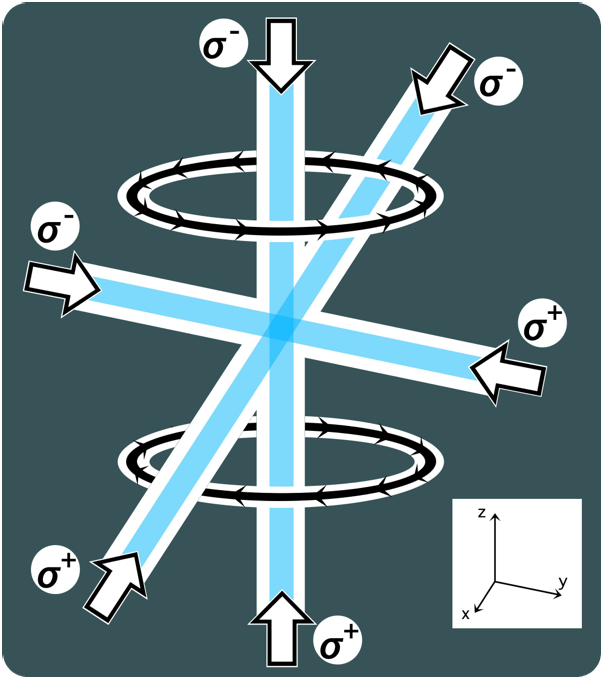
\includegraphics[width=\textwidth]{mot.png}
		%	\label{fig:mot}
			\caption{Components of a magneto-optical trap, including current-carrying magnetic field coils and counterpropagating circularly polarized laser beams.}
			\label{fig:mot}
		\end{subfigure}
		\hfill
	%	\begin{subfigure}[t]{0.726\textwidth}
		\begin{subfigure}[t]{0.728\textwidth}
			\centering
			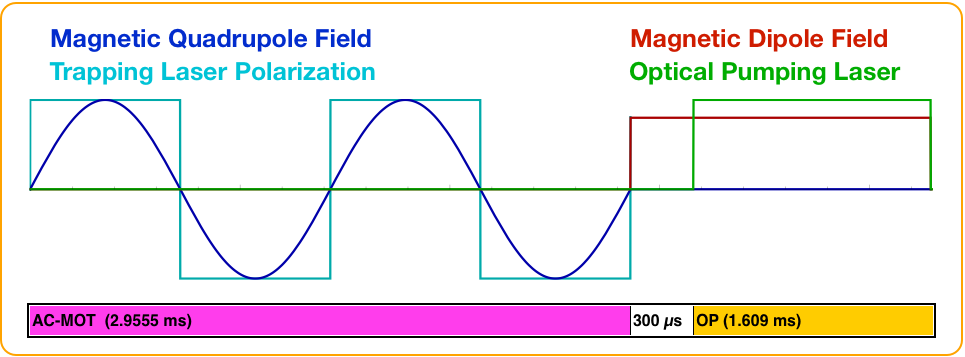
\includegraphics[width=\textwidth]{acmot.png}
			\caption{One cycle of trapping with the AC-MOT, followed by optical pumping to spin-polarize the atoms.  After atoms are transferred into the science chamber, this cycle is repeated 500 times before the next transfer.  The magnetic dipole field is created by running parallel (rather than anti-parallel as is needed for the MOT) currents through the two coils.}
			\label{fig:acmot}
		\end{subfigure}
		\caption{An alternating-current magneto-optical trap with a duty cycle optimized for producing polarized atoms}	
		\label{fig:themot}
	\end{figure}
	
	
	
%	\subsection{\textbf{Nuclear Setup}}
\section{Measurement Geometry and Detectors}
	%\\*
	Needs several diagrams.  Back-to-back beta detectors along the polarization axis.  Back-to-back MCPs in an electric field to tag events from the trap, and to measure the trap position and polarization.  Hoops to produce the electric field.  Many laser ports to make the MOT functional, and for optical pumping.  Fancy mirror geometry to combine optical pumping and trapping light along the vertical axis.  Water-cooled (anti-)Helmholz coils within the chamber for the AC-MOT, fast switching to produce an optical pumping field.  
%	\subsection{\textbf{All the Detectors}}


%%%% --- * --- %%%%	
\clearpage	
\chapter{Calibrations}
\label{calibrations_chapter}
	
\section{Polarization}
	%\\*
	Polarization measurement was conducted on a different set of data, collected in between the measurements used for $A_{\mathrm{\beta}}$ and $b_{\mathrm{Fierz}}$, and at a higher electric field, because we were unable to run both our MCP detectors simultaneously.  
	
\section{Trap Position}
	%\\*
	Measured using the same dataset that was used to quantify the polarization.  The trap drifts slightly over the course of our data collection.  Describe the rMCP calibration needed to extract this info.  
	
\section{Beta Detectors}
	%\\*
	Energy calibration for the scintillator+PMT setup changed dramatically at one point.    Describe how calibration was done.  Also describe how the DSSD calibration was done, even though it wasn't implemented by me.  
	
\section{The eMCP}
	%\\*
	I can describe the eMCP calibration here, even though it mostly wasn't implemented by me.  It is tangentially relevant to data selection and background estimation by providing an experimental energy spectrum for shake-off electrons.  
	
	
%%%% --- * --- %%%%	
\clearpage	
%\part{Data Analysis}
%\section{The Experimental Signature}
\chapter{The Experimental Signature}
\label{analysis_chapter}

\section{The Superratio and Asymmetry}
	%\\*
	The data can be combined into a superratio asymmetry.  This has the benefit of causing many systematics to cancel themselves out at leading order.  It also will increase the fractional size of the effects we're looking for.  This can be shown by using math.  
	
\section{Signature of a Fierz Term in This Experiment}
	%\\*
	Not all systematics effects are eliminated.  We'll want to be careful to propagate through any effects that are relevant.  Using the superratio asymmetry as our physical observable makes this process a bit messier for the things that don't cancel out, but it's all just math.  
	
\section{Comparative Merits of the Superratio and Supersum for Measurement}
	%\\*
	Some other groups have performed similar measurements using the supersum as the physical observable.  There are pros and cons to both methods.  I can show, using a back-of-the-envelope calculation, that for this particular dataset, the superratio asymmetry method produces a better result.  
	

\chapter{Estimating Systematic Effects}
	\section{Low-energy Scintillator Threshold}
	%\\*
	Choice of low-energy scintillator threshold has a large systematic effect...  
	
	\section{BB1 Radius, Energy Threshold, Agreement}
	%\\*
	BB1 radius cut can help to eliminate scattered events.  Energy threshold selection and statistical agreement between BB1 detectors' energies only makes a small effect on results.  

\section{Background Modeling}
	\subsection{Decay from Chamber Surfaces}

\section{Quantifying the Effects Backscatter with Geant4}
	Beta decay (back-)scatter from surfaces within the experimental chamber is a significant systematic, and it must be evaluated, quantified, and corrected for.  This is done via a series of GEANT4 simulations.  While only a small fraction of events are affected, the process results in an energy loss in the beta that can, if not understood, be misinterpreted as the exact signal we're searching for.  It is therefore imperative that this be well understood. 

\section{Lineshape Reconstruction}
	\subsection{Motivation}
	This process is used because the (back-)scatter, which it itself an important systematic, is largely independent of a wide variety of other experimental effects.  These other effects must all be evaluated, but it is computationally prohibitive to re-evaluate the scattering with every other effect under consideration.
	
	\subsection{What is it and how does it work?}
	Mono-energetic beta decay events are generated in GEANT4, which outputs an energy spectrum for unscattered and forward-scattered beta events in the detector.  These spectra are fit to a function to model the scintillator resolution, as well as energy loss in materials that the beta passed through before arriving at the scintillator.  These spectrum fits are performed for a set of beta energies, and parameters are extrapolated to be applied to betas emitted at intermediate energies.  Thus, the whole spectrum can be modeled.  Pictures will make this clearer. 
	
	\subsection{The Math-Specifics}
	I'll write down the specific functions I'm using, and the parameter values I'm using.  (Maybe this should go in an appendix instead?)  I'll describe the adjustments I make to the spectrum so that it can work even for the dataset where the scintillators' resolutions have changed.
	
	\subsection{The Results -- Things That Got Evaluated This Way}
	Trap position, size, sail velocity.  Thicknesses of the SiC mirror, the Be foil, and the DSSD.  Scintillator calibration.  
	
	\subsection{The low-energy tail uncertainty, and what it does}


%%%% --- * --- %%%%	
\clearpage	
%\part{Results}
\chapter{Results}

\section{Measured Limits on $b_{Fierz}$, $C_S$, $C_T$}
	%\\*
	Results go here, with measured limits described and quantified in all formats anyone could ever care about.
	
\section{Discussion of Corrections and Uncertainties}
	...
	
\section{Relation to Other Measurements and New Overall Limits}
	%\\*
	In which I'll show exclusion plots and write down new limits, combining my result with results from the literature.


